% Diagrama de bloques del emisor-receptor y de la validación en el receptor.
% Compilar: pdflatex diagrama_bloques_receptor.tex
\documentclass[tikz,border=6pt]{standalone}
\usepackage[utf8]{inputenc}
\usepackage[T1]{fontenc}
\usepackage{helvet}
\renewcommand{\familydefault}{\sfdefault}
\usepackage{courier}
\usetikzlibrary{positioning,arrows.meta,fit,backgrounds,calc}

\begin{document}
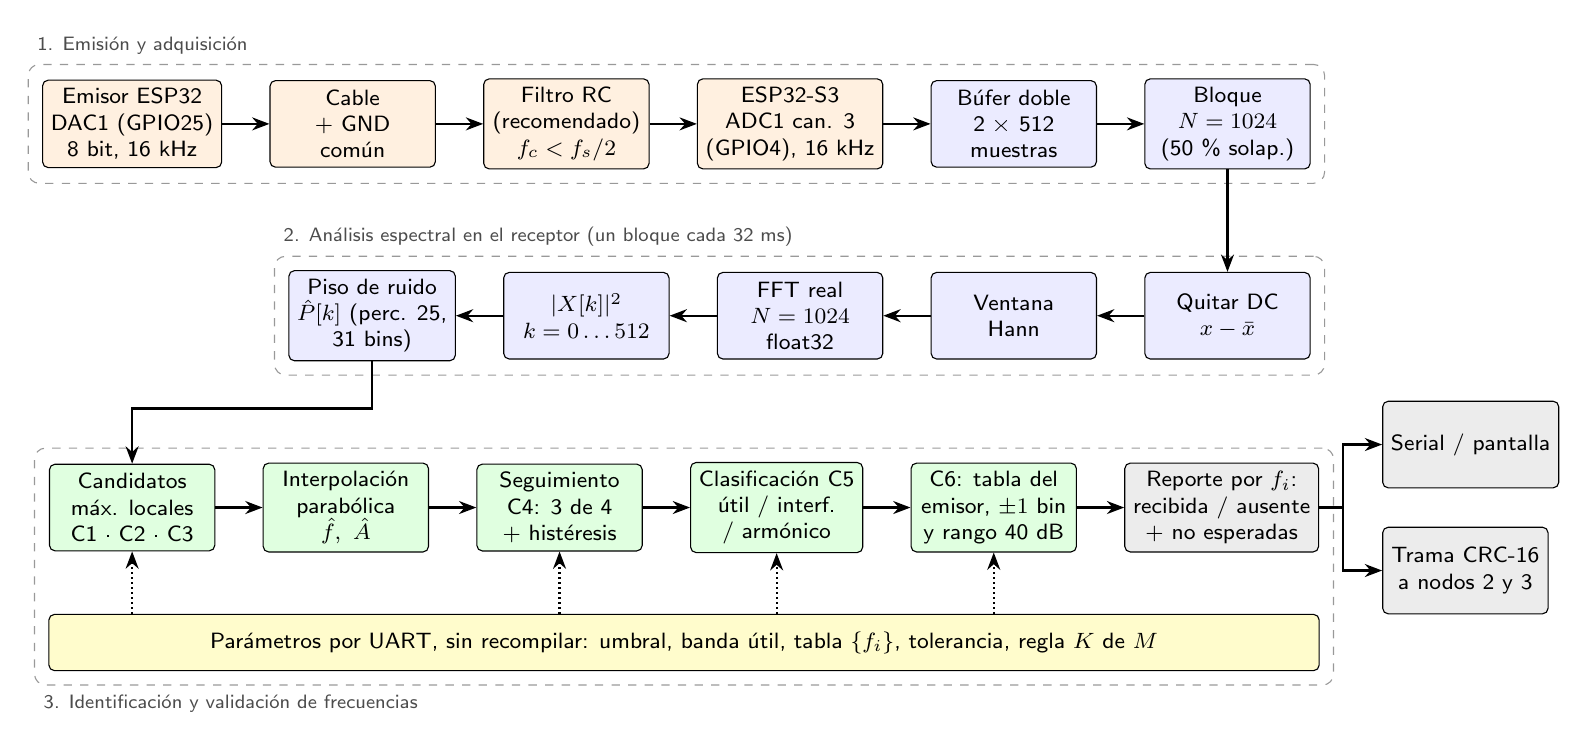
\begin{tikzpicture}[
  font=\footnotesize,
  >={Stealth[length=2.2mm]},
  bloque/.style={draw, rounded corners=2pt, fill=white, align=center,
                 minimum height=11mm, minimum width=21mm, inner sep=3pt},
  analog/.style={bloque, fill=orange!12},
  dsp/.style={bloque, fill=blue!8},
  decision/.style={bloque, fill=green!12},
  com/.style={bloque, fill=gray!15},
  linea/.style={->, thick},
  nota/.style={font=\scriptsize, text=black!70, align=center},
  grupo/.style={draw=black!40, dashed, rounded corners=4pt, inner sep=5pt}
]

% ---- Fila 1: emisor y adquisición ----------------------------------------
\node[analog] (emi) {Emisor ESP32\\DAC1 (GPIO25)\\8 bit, 16 kHz};
\node[analog, right=6mm of emi] (sig) {Cable\\+ GND\\común};
\node[analog, right=6mm of sig] (aa) {Filtro RC\\(recomendado)\\$f_c < f_s/2$};
\node[analog, right=6mm of aa] (adc) {ESP32-S3\\ADC1 can. 3\\(GPIO4), 16 kHz};
\node[dsp, right=6mm of adc] (dma) {Búfer doble\\2 × 512\\muestras};
\node[dsp, right=6mm of dma] (blk) {Bloque\\$N = 1024$\\(50 \% solap.)};

\draw[linea] (emi) -- (sig);
\draw[linea] (sig) -- (aa);
\draw[linea] (aa) -- (adc);
\draw[linea] (adc) -- (dma);
\draw[linea] (dma) -- (blk);

% ---- Fila 2: análisis espectral ------------------------------------------
\node[dsp, below=13mm of blk] (dc) {Quitar DC\\$x - \bar{x}$};
\node[dsp, left=6mm of dc] (win) {Ventana\\Hann};
\node[dsp, left=6mm of win] (fft) {FFT real\\$N=1024$\\float32};
\node[dsp, left=6mm of fft] (pot) {$|X[k]|^2$\\$k=0\ldots512$};
\node[dsp, left=6mm of pot] (piso) {Piso de ruido\\$\hat P[k]$ (perc. 25,\\31 bins)};

\draw[linea] (blk) -- (dc);
\draw[linea] (dc) -- (win);
\draw[linea] (win) -- (fft);
\draw[linea] (fft) -- (pot);
\draw[linea] (pot) -- (piso);

% ---- Fila 3: identificación y validación ---------------------------------
\node[decision, anchor=north] (cand) at ($(emi |- piso.south)+(0,-13mm)$) {Candidatos\\máx. locales\\C1 · C2 · C3};
\node[decision, right=6mm of cand] (interp) {Interpolación\\parabólica\\$\hat f,\ \hat A$};
\node[decision, right=6mm of interp] (pers) {Seguimiento\\C4: 3 de 4\\+ histéresis};
\node[decision, right=6mm of pers] (clas) {Clasificación C5\\útil / interf.\\/ armónico};
\node[decision, right=6mm of clas] (tabla) {C6: tabla del\\emisor, $\pm 1$ bin\\y rango 40 dB};
\node[com, right=6mm of tabla] (rep) {Reporte por $f_i$:\\recibida / ausente\\+ no esperadas};

\draw[linea] (piso.south) -- ++(0,-6mm) -| (cand.north);
\draw[linea] (cand) -- (interp);
\draw[linea] (interp) -- (pers);
\draw[linea] (pers) -- (clas);
\draw[linea] (clas) -- (tabla);
\draw[linea] (tabla) -- (rep);

% ---- Salidas --------------------------------------------------------------
\node[com, right=8mm of rep, yshift=8mm] (ser) {Serial / pantalla};
\node[com, right=8mm of rep, yshift=-8mm] (nod) {Trama CRC-16\\a nodos 2 y 3};
\draw[linea] (rep.east) -- ++(3mm,0) |- (ser.west);
\draw[linea] (rep.east) -- ++(3mm,0) |- (nod.west);

% Parámetros ajustables sin recompilar.
\coordinate (cfgA) at ($(cand.south west)+(0,-8mm)$);
\coordinate (cfgB) at ($(rep.south east)+(0,-15mm)$);
\node[draw, rounded corners=2pt, fill=yellow!20, fit=(cfgA)(cfgB), inner sep=0pt,
      label={[font=\footnotesize]center:Parámetros por UART, sin recompilar:
      umbral, banda útil, tabla $\{f_i\}$, tolerancia, regla $K$ de $M$}] (cfg) {};
\foreach \dest in {cand, pers, clas, tabla}
  \draw[linea, densely dotted] (\dest.south |- cfg.north) -- (\dest.south);

% Grupos por etapa
\begin{scope}[on background layer]
  \node[grupo, fit=(emi)(sig)(aa)(adc)(dma)(blk),
        label={[nota, anchor=south west]north west:1. Emisión y adquisición}] {};
  \node[grupo, fit=(dc)(win)(fft)(pot)(piso),
        label={[nota, anchor=south west]north west:2. Análisis espectral en el receptor (un bloque cada 32 ms)}] {};
  \node[grupo, fit=(cand)(interp)(pers)(clas)(tabla)(rep)(cfg),
        label={[nota, anchor=north west]south west:3. Identificación y validación de frecuencias}] {};
\end{scope}

\end{tikzpicture}
\end{document}
